\documentclass[12pt]{article}
\usepackage{amrl}% This is the style for AMRL full report
% \usepackage[margin=1.5cm]{geometry}
\usepackage{graphicx}
\usepackage{amsmath}
\usepackage{amsfonts}
\usepackage{amssymb}
\usepackage{url}
\usepackage{natbib}
\usepackage{xcolor}
\usepackage{setspace}
\usepackage{graphicx}
\usepackage{subfig}
\usepackage{multirow}
\usepackage{float}
\usepackage{caption}
\usepackage{mathbbol}
\newtheorem{Def}{Definition}
\newtheorem{Thm}{Theorem}
\newtheorem{Exmp}{Example}

\DeclareMathOperator*{\argmax}{arg\,max}
\DeclareMathOperator*{\argmin}{arg\,min}

%command to highlight a block of text in color
\newcommand{\highlight}[2][blue]{{\color{#1}{#2}}}
\graphicspath{{./images}}



\hoffset -6mm
\voffset -7mm
\textwidth 16cm
\textheight 22cm

\title{CenterNet - A comparison of CenterNet with \\
other state-of-the-art methods in object detection} 
\author{Nong Minh Hieu\\ \\
 School of Computing and Information Technology\\
 University of Wollongong}

\abstract{
This report explores the proposed method in the "Object as Points" paper along with some of the visualization results from evaluating CenterNet as compared with YoloV3. The pretrained models used in this evaluation is taken from GluonCV - an extended deep learning library for Apache MxNet.
}

\email{mhmn546@uowmail.edu.au}

\onehalfspacing

\begin{document}
\maketitle

\section*{Introduction}

CenterNet is an interesting research in the topic of anchor-free detection methods. Unlike the predecessors in the domain like Yolo, the RCNN family or RetinaNet, CenterNet treats object detection problem as a keypoint estimation problem which finds the center points and use them to regress the rest of the object properties (dimensions, 3D locations, orientations and poses). This removes the exhaustive proposal of bounding boxes which is often inefficient and wasteful due to the fact that most of the potential regions are classified as non-objects. In this report, I will explore the fundamental intuitions behind CenterNet and present some of the visualization results that evaluates the performance of CenterNet as compared to YoloV3 - on of CenterNet's predecessors.\newline


\textit{The mathematical details of how the loss functions are formulated, the training procedures and optimization method are outside the scope of this report}


\section*{Intuition}
In the training time, the input is initially forward through a feature extraction architecture. In the original paper, the experimented architectures include HourGlass-104, ResNet-18, ResNet-101 and DLA-34. The feature map is then directed through three output channels (heads) which are called the Heatmap Head, the Dimension Head and the Offset Head. The heatmap head defines the confidence of the objectness in each location and the local peaks of the heatmaps are used as predicted center points. The Dimension Head predicts object properties like width and height. The Offset Head is used to recover from the discretization error caused by downsampling the input image.

\begin{figure}[H]
    \centering
    \captionsetup{justification=centering}
    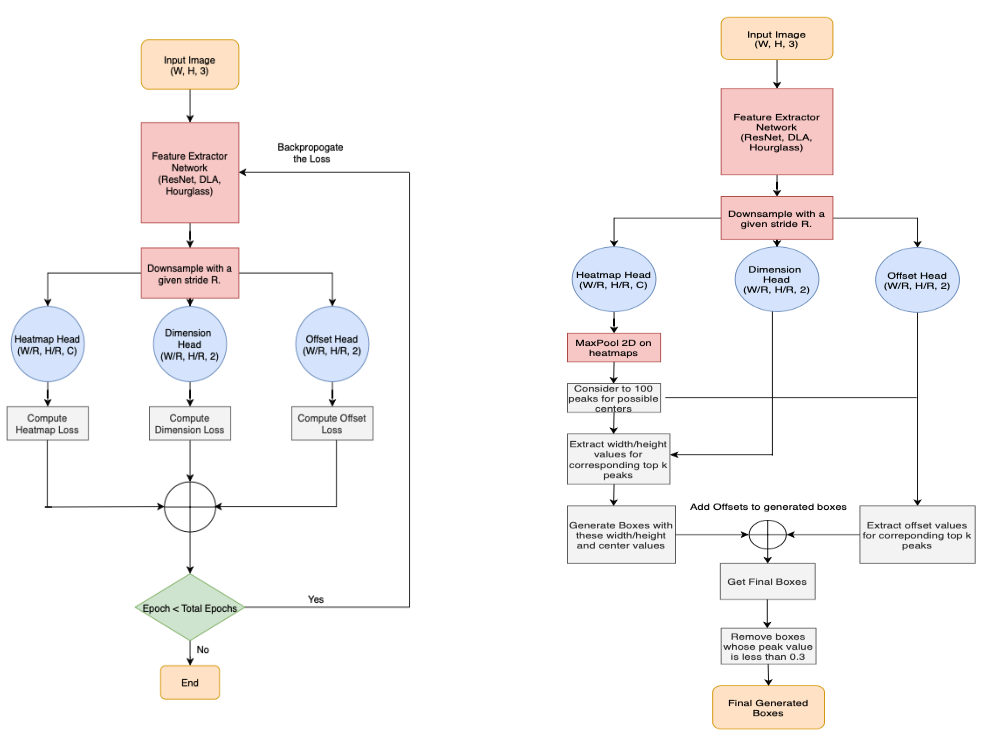
\includegraphics[scale=0.35]{./images/CenterNet_flow.png}
    \caption{CenterNet workflow in training time (left) and inference time (right)}
\end{figure}



\textbf{Note (Heatmap Head)} - To generate the ground truth for training the Heatmap Head, the ground truth center point is splashed onto a $\mathbb{R}^{\frac{W}{R}\times\frac{H}{R}\times C}$ matrix using a Gaussian Kernel :

\begin{align}
    Y_{xyc}=exp(-\frac{(x- \tilde p_x)^2 + (y - \tilde p_y)^2}{2\sigma_p^2})
\end{align}

Where H and W are the dimensions of the original input image, C is the number of classes (80 in case of COCO dataset), R is the output stride, $(\tilde p_x, \tilde p_y)$ is the coordinate of the ground truth center points and $\sigma_p$ controls how "spreaded" your splash of the center points is. 

\begin{figure}[H]
    \centering
    \captionsetup{justification=centering}
    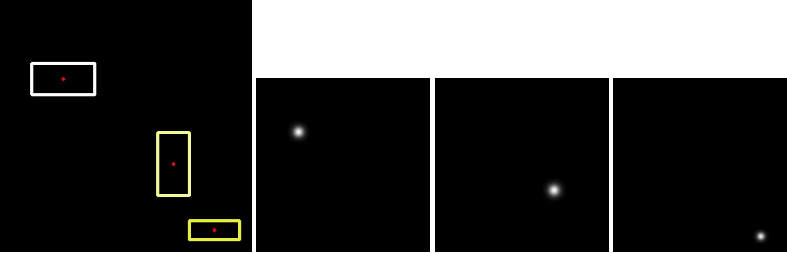
\includegraphics[scale=0.35]{./images/splash.png}
    \caption{Ground-truth center points of different classes splashed onto the heatmap using the Gaussian Kernel}
\end{figure}

\section*{CenterNet and YoloV3 comparison}
In order to attain an objective comparison between CenterNet and other state-of-the-art methods, I used the pretrained CenterNet and pretrained YoloV3 models derived from the model zoo of GluonCV, an extended deep learning library for Apache MxNet. Both of the models are trained on the same benchmark which is the COCO open dataset comprises of 80 different classes. The evaluation metrics consist of Frame Per Second (FPS), Detection Rate (Objects per frame), Precision and Recall trade-off and mean Average Precision (mAP).

\subsection*{1. Real-time detection performance}
In the original paper, the authors claimed that the proposed CenterNet acquires real-time detection performance that rivals the contemporary state-of-the-arts like YoloV3, RetinaNet and Faster-RCNN. To verify this, an evaluation script is ran for both YoloV3 and CenterNet on three testing videos. The evaluation metrics are then calculated and visualized.\newline

\textbf{Frames Per Second (FPS)} : This metric measures the inference speed in real-time. It defines how many frames each model can process in a second.
\begin{figure}[H]
    \centering
    \captionsetup{justification=centering}
    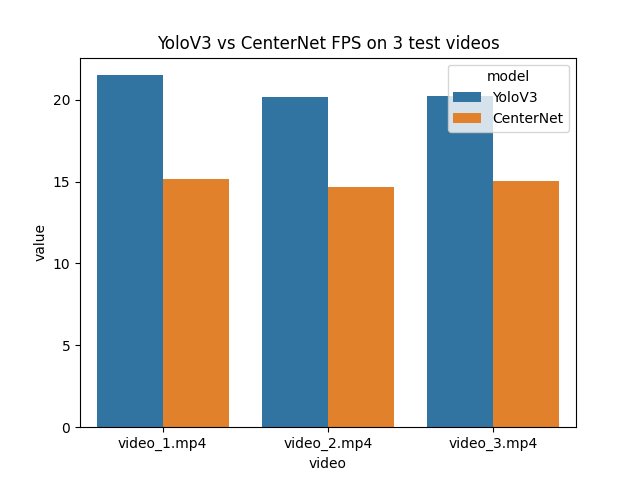
\includegraphics[scale=0.8]{images/fps_yolo_vs_centernet.png}
    \caption{FPS of CenterNet and YoloV3 measured on three different testing videos}
\end{figure}

It can be seen from Figure 3 that unlike the original claim of the "Object as Points" paper, the experiment results showed that YoloV3 out-performed CenterNet in all three evaluating videos by a slight margin.\newline

\textbf{Detection Rate} : This metric measures the model's ability to capture correctly as many objects as possible. It defines how many objects a model can capture in a frame given a  confidence threshold. In this experiment, the threshold is set at 0.6.

\begin{figure}[H]
    \centering
    \captionsetup{justification=centering}
    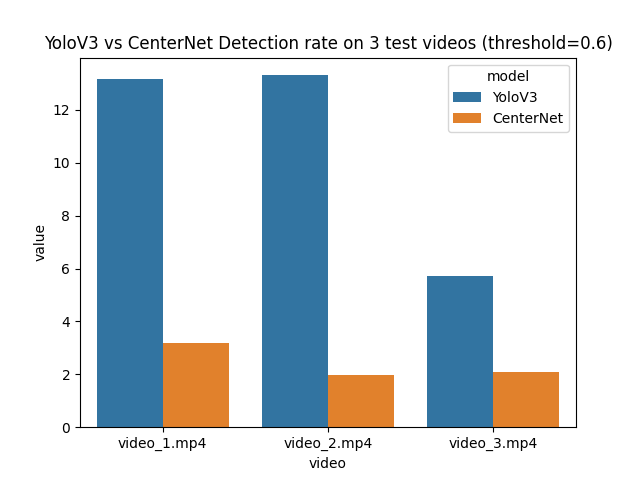
\includegraphics[scale=0.8]{images/dr_yolo_vs_centernet.png}
    \caption{Detection rate of CenterNet and YoloV3 measured on three different testing videos}
\end{figure}

It can be seen from Figure 4 that the evaluation using detection rate (objects per frame) showed a wider gap in performance where YoloV3 triumphs CenterNet by a larger margin as compared to the evaluation on FPS. 

\subsection*{2. Precision and Recall trade-off}
To increase the objectivity of the evaluation, I tested both models on a different dataset other than the provided three testing videos. The dataset is sampled from Vehicles-OpenImages dataset which comprises of different vechicle classes like ambulance, truck, car, bus and motorcycle. To preserve the consistency of the evaluation, the ambulance class is removed since this class is not included in the COCO open dataset which both models are trained on.

\begin{figure}[H]%
    \centering
    \subfloat[\centering PR curve - CenterNet]{{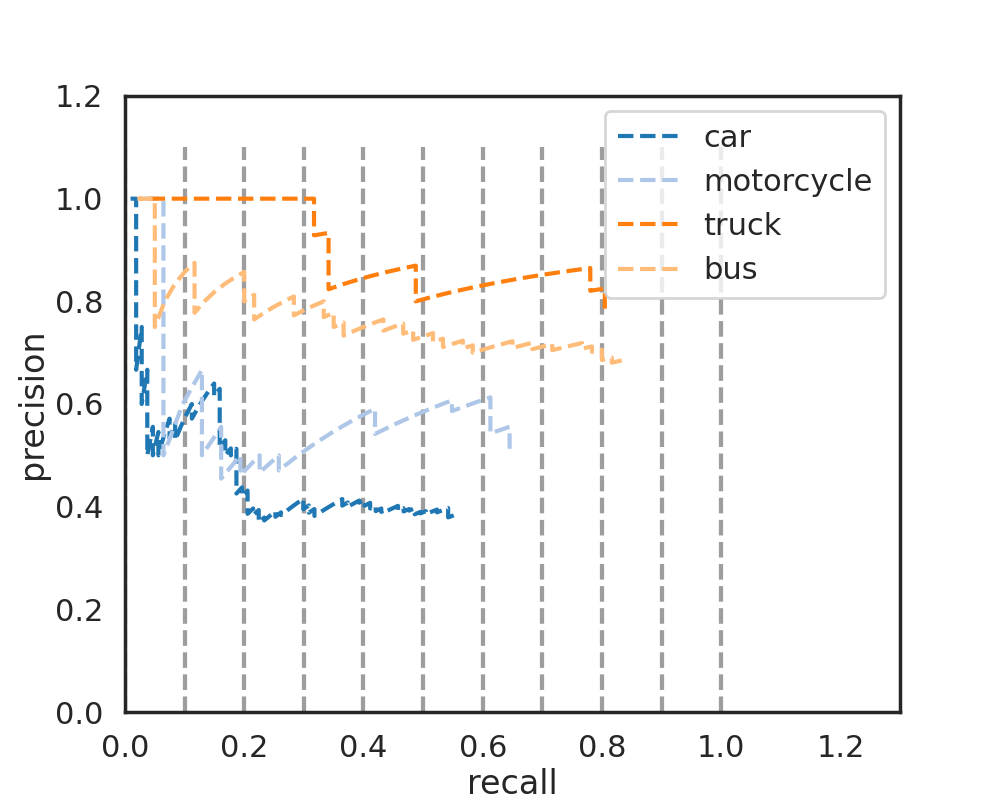
\includegraphics[width=7cm]{images/pr_center.png} }}%
    \qquad
    \subfloat[\centering PR curve - YoloV3]{{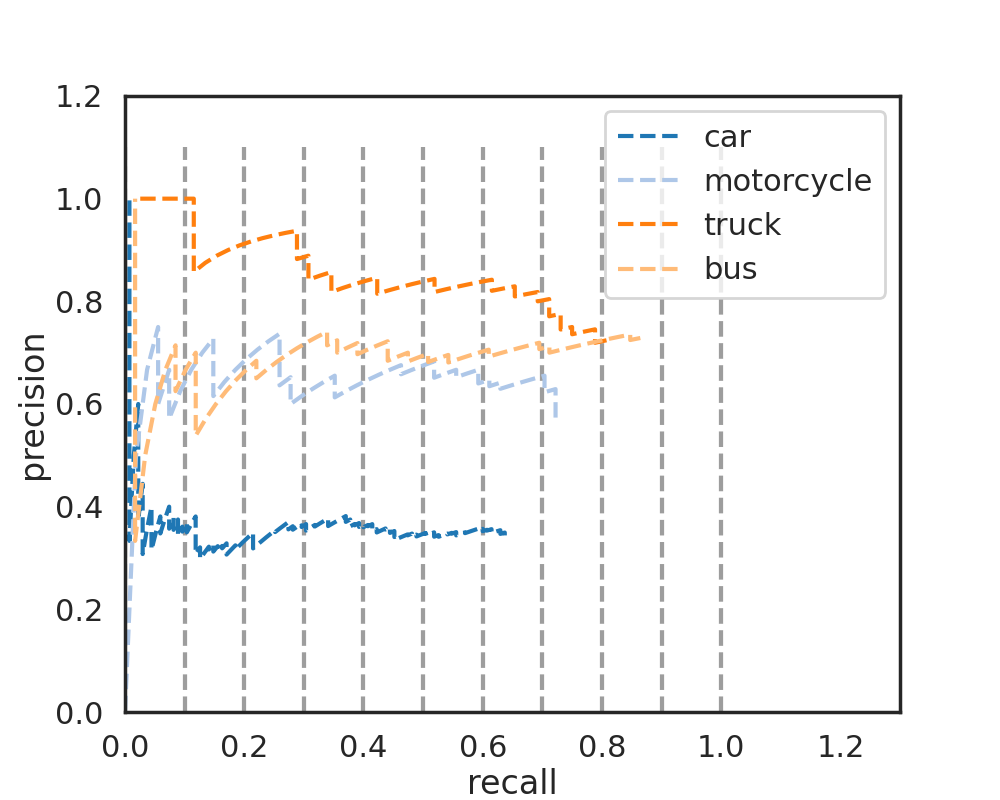
\includegraphics[width=7cm]{images/pr_yolo.png} }}%
    \caption{Precision and recall trade-off of CenterNet and YoloV3 on each individual class}%
    \label{fig:example}%
\end{figure}

In this evaluation, I used the IOU threshold of 0.6 and probability score threshold of 0.6 (the same as done in evaluation on the videos) to calculate the precision-recall trade-off of both models. The visual proof indicates that in this case, CenterNet offers a better trade-off for most of the object classes (Truck, Bus and Car). To further back this point, I calculated the average precision of each model on different IOU thresholds and use the mean Average Precision to finalize the measurement.\newline

\begin{center}
\begin{tabular}{ |c|c|c|c|c| } 
\hline
Model & Car & Truck & Bus & Motorcycle \\
\hline
CenterNet & \textbf{0.39} & \textbf{0.76} & \textbf{0.69} & 0.46 \\ 
YoloV3 & 0.30 & 0.71 & 0.61 & \textbf{0.50} \\ 
\hline
\end{tabular}
\end{center}

The discrepancy in performance between the evaluations in the videos data and in the images data can be attributed to the fact that the objects presented in the image dataset is of a closer perspective as compared to the videos. From this point, it can be concluded that CenterNet is more suitable for close range detection.

\section*{Limitations of CenterNet}
\subsection*{1. Center points collision}
As mentioned in the original paper, the evaluation results on the COCO open dataset showed that there were 614 pairs of objects that collided onto the same center point at stride 4. However, the authors justified that this accounted for less than 0.1\% of the overall dataset and this error rate is acceptable. Nonetheless, center points collision is still a considerable issue when it comes to detecting high density of objects and it suggests that Yolo is still a more robust choice when it comes down to varying environmental conditions.

\begin{figure}[H]%
    \centering
    \subfloat[\centering CenterNet]{{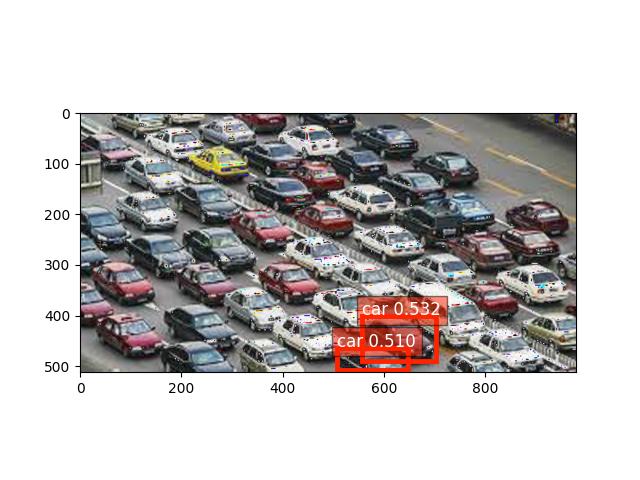
\includegraphics[width=7cm]{images/collide_centernet.png} }}%
    \qquad
    \subfloat[\centering YoloV3]{{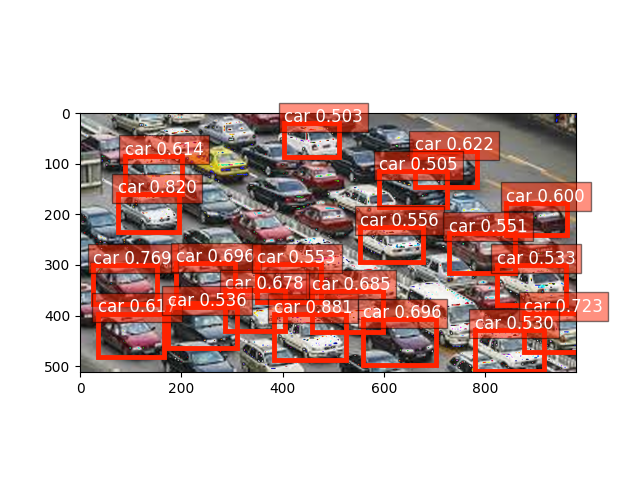
\includegraphics[width=7cm]{images/collide_yolo.png} }}%
    \caption{Detection result in high density of objects: CenterNet vs. YoloV3}%
    \label{fig:example}%
\end{figure}

\subsection*{2. Performance}
As presented in the comparison between YoloV3 and CenterNet in terms of real-time performance, the novelty of the proposed result is questionable. While the proposed CenterNet did successfully get rid of the hustle from bounding boxes proposal, in inference time, the intermediate operations (Heatmap peaks filtering, dimensions extraction and offset correction) still take up a lot of processing time. This can be a real hindrance in the case where a lot of objects are present in the image. Unlike Yolo where the objectness score, class probabilities and bounding box coordinates are infered in a single-shot detection manner.

\section*{Conclusion}


\bibliographystyle{agsm} 
\bibliography{amrl_full_report}

\end{document}

